\section{Basic Concepts}

\begin{frame}{What is Frequent-pattern Analysis?}

	\begin{block}{Frequent Pattern}
		A pattern (a set of items, subsequences, substructures, etc.) that occurs frequently in a dataset.
	\end{block}
	\begin{itemize}
		\item \textbf{Finding inherent regularities in data:}
		      \begin{itemize}
			      \item What products are often purchased together? Beer and diapers?!
			      \item What are the subsequent purchases after buying a PC?
			      \item Who bought this has often also bought $\ldots$
			      \item What kinds of DNA are sensitive to this new drug?
			      \item Can we automatically classify web documents?
		      \end{itemize}
	\end{itemize}

	\vspace{0.5cm}

	\only<2->{
		\begin{alertblock}{Intrinsic and Important}
			A frequent pattern is an intrinsic and important property of a dataset.
		\end{alertblock}
	}
\end{frame}

\newcommand{\smartphone}[2][]{
	% Note: The dimensions of this wrapper are matched to the screenshot ratio of an iPhone 16 Pro Max (1320x2868)
	%	    It might be necessary to adjust this ratio for screenshots of other devices.

	\begin{tikzpicture}[#1]
		\draw[rounded corners=10pt, line width=1pt, fill=faugray!10]
		(0,0) rectangle (6,13.52);

		\draw[rounded corners=5pt, line width=0.5pt, fill=white]
		(0.3,0.8) rectangle (5.7,12.52);

		\begin{scope}
			\clip[rounded corners=5pt] (0.3,0.8) rectangle (5.7,12.52);
			\node[anchor=center, inner sep=0pt] at (3,6.66)
			{\includegraphics[width=5.4cm]{#2}};
		\end{scope}

		\draw[line width=0.5pt, fill=white] (3,0.4) circle (0.25);

		\draw[rounded corners=1pt, fill=faugraydark!50] (2.5,12.82) rectangle (3.5,13.02);

	\end{tikzpicture}
}

\begin{frame}
	\frametitle{Some Real World Examples}

	\begin{center}
		\scalebox{0.45}{
			\smartphone{img/frequent-patterns-shopping.png}

			\hspace*{2cm}

			\smartphone{img/frequent-patterns-education.png}

			\hspace*{2cm}

			\smartphone{img/frequent-patterns-movies.png}
		}
	\end{center}

	\vspace{-2.15cm}

	\only<2->{
		\begin{block}{Recommendation Systems}
			While frequent pattern analysis often serves as the \textbf{foundation} of recommendation systems, such systems typically consist of multiple distinct components.
		\end{block}
	}
\end{frame}

\begin{frame}{Why is Frequent-pattern Mining Important?}
	\begin{itemize}
		\item \textbf{Foundation for many essential data-mining tasks:}
		      \begin{itemize}
			      \item Association, correlation, and causality analysis.
			      \item Sequential, structural (e.g., sub-graph) patterns.
			      \item Pattern analysis in spatiotemporal, multimedia, time-series,
			            and stream data.
			      \item Classification: discriminative, frequent-pattern analysis.
			      \item Cluster analysis: frequent-pattern-based clustering.
			      \item Data warehousing: iceberg cube and cube gradient.
			      \item Semantic data compression: fascicles\footnote{\fullcite{jagadish1999}}
			      \item Broad applications.
		      \end{itemize}
	\end{itemize}
\end{frame}

\begin{frame}{Basic Concepts: Frequent Itemsets}
	\begin{itemize}
		\item \textbf{Itemset:}
		      \begin{itemize}
			      \item A set of one or more items.
			      \item $k$-itemset $X = \{x_1, x_2, \ldots, x_k\}$.
		      \end{itemize}
		\item \textbf{Support:}
		      \begin{itemize}
			      \item \textbf{Absolute Support} $s$/\textbf{Support Count} of $X$:
			            \begin{itemize}
				            \item Frequency or occurrence count of $X$.
			            \end{itemize}
			      \item \textbf{Relative Support} $s$:
			            \begin{itemize}
				            \item The fraction of the transactions that contain $X$.
				            \item I.e. the \textbf{probability} that a transaction
				                  contains $X$.
			            \end{itemize}
		      \end{itemize}
	\end{itemize}

	\vspace*{0.75cm}

	\begin{block}{Frequent Itemset}
		An itemset $X$ is frequent, if $X$'s support is no less than a \texttt{min\_sup} threshold.
	\end{block}
\end{frame}

\begin{frame}{Frequent Itemsets - Example}
	\begin{columns}
		\begin{column}{0.4\textwidth}
			\begin{tabular}{|c|c|}
				\hline
				\textbf{TID} & \textbf{Items bought}             \\\hline
				10           & Beer, Nuts, Diapers               \\\hline
				20           & Beer, Coffee, Diapers             \\\hline
				30           & Beer, Diapers, Eggs               \\\hline
				40           & Nuts, Eggs, Milk                  \\\hline
				50           & Nuts, Coffee, Diapers, Eggs, Milk \\\hline
			\end{tabular}
			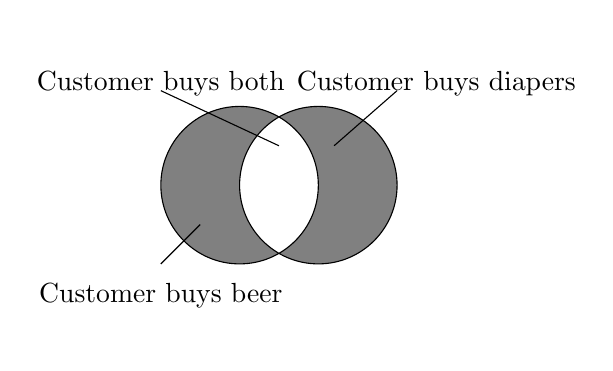
\begin{tikzpicture}[fill=gray]
				% left hand
				\scope
				\clip (-2,-2) rectangle (2,2)
				(1,0) circle (1);
				\fill (0,0) circle (1);
				\endscope
				% right hand
				\scope
				\clip (-2,-2) rectangle (2,2)
				(0,0) circle (1);
				\fill (1,0) circle (1);
				\endscope
				% outline
				\draw (0,0) circle (1) (0,1) (1,0) circle (1) (1,1);
				\node[label=below:{Customer buys beer}] at (-1,-1) {};
				\node[label=below:{Customer buys diapers}] at (2.5,1.7) {};
				\node[label=below:{Customer buys both}] at (-1,1.7) {};
				\draw (-1,-1) -- (-0.5,-0.5);
				\draw (2,1.2) -- (1.2,0.5);
				\draw (-1,1.2) -- (0.5,0.5);
			\end{tikzpicture}
		\end{column}
		\begin{column}{0.5\textwidth}
			\vspace{-1.25cm}
			\begin{itemize}
				\item \textbf{Minimum (absolute) support threshold:}
				      \begin{itemize}
					      \item Set by the user.
					      \item In this example: $min\_sup = 3$.
				      \end{itemize}
				\item \textbf{Frequent Itemsets:}
				      \begin{itemize}
					      \item \textbf{1-itemsets:}
					            \begin{itemize}
						            \item \only<2->{\{Beer\}: $3$, \{Nuts\}: $3$, \{Diapers\}: $4$, \{Eggs\}: $3$.}
					            \end{itemize}
					      \item \textbf{2-itemsets:}
					            \begin{itemize}
						            \item \only<3->{\{Beer, Diapers\}: $3$}
					            \end{itemize}
					      \item \textbf{3-itemsets:}
					            \begin{itemize}
						            \item \only<4->{\textit{None}}
					            \end{itemize}
					      \item \textbf{4-itemsets:}
					            \begin{itemize}
						            \item \only<5->{\textit{None}}
					            \end{itemize}
					      \item \textbf{5-itemsets:}
					            \begin{itemize}
						            \item \only<6->{\textit{None}}
					            \end{itemize}
				      \end{itemize}
			\end{itemize}
		\end{column}
	\end{columns}
\end{frame}

\begin{frame}{Basic Concepts: Association Rules}
	\begin{itemize}
		\item \textbf{Implication of the form $A \implies B$:}
		      \begin{itemize}
			      \item where $A \neq \emptyset$, $B \neq \emptyset$ and $A \cap B =
				            \emptyset$.
		      \end{itemize}
		\item \textbf{Strong rule:}
		      \begin{itemize}
			      \item Satisfies both $\text{min\_sup}$ and $\text{min\_conf}$
			            \begin{align*}
				            \text{support}(A \implies B)    & = P(A \cup B),                                        \\
				            \text{confidence}(A \implies B) & = P(B | A)                                            \\
				                                            & = \frac{\text{support}(A \cup B)}{\text{support}(A)}.
			            \end{align*}
			      \item I.e. confidence of rule can be easily derived from the
			            support counts of $A$ and $A \cup B$.
		      \end{itemize}
		\item \textbf{Association-rule mining:}
		      \begin{itemize}
			      \item Find all frequent itemsets (with a length of at least $2$).
			      \item Generate strong association rules from the frequent itemsets.
		      \end{itemize}
	\end{itemize}
\end{frame}

\begin{frame}{Association Rules - Example}
	\begin{columns}
		\begin{column}{0.4\textwidth}
			\begin{tabular}{|c|c|}
				\hline
				\textbf{TID} & \textbf{Items bought}             \\\hline
				10           & Beer, Nuts, Diapers               \\\hline
				20           & Beer, Coffee, Diapers             \\\hline
				30           & Beer, Diapers, Eggs               \\\hline
				40           & Nuts, Eggs, Milk                  \\\hline
				50           & Nuts, Coffee, Diapers, Eggs, Milk \\\hline
			\end{tabular}
			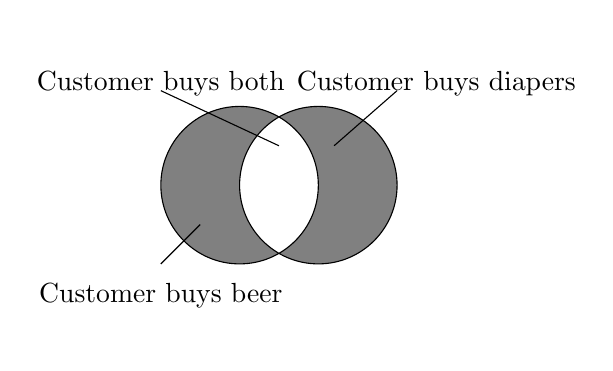
\begin{tikzpicture}[fill=gray]
				% left hand
				\scope
				\clip (-2,-2) rectangle (2,2)
				(1,0) circle (1);
				\fill (0,0) circle (1);
				\endscope
				% right hand
				\scope
				\clip (-2,-2) rectangle (2,2)
				(0,0) circle (1);
				\fill (1,0) circle (1);
				\endscope
				% outline
				\draw (0,0) circle (1) (0,1) (1,0) circle (1) (1,1);
				\node[label=below:{Customer buys beer}] at (-1,-1) {};
				\node[label=below:{Customer buys diapers}] at (2.5,1.7) {};
				\node[label=below:{Customer buys both}] at (-1,1.7) {};
				\draw (-1,-1) -- (-0.5,-0.5);
				\draw (2,1.2) -- (1.2,0.5);
				\draw (-1,1.2) -- (0.5,0.5);
			\end{tikzpicture}
		\end{column}
		\begin{column}{0.5\textwidth}
			\vspace{-1.25cm}
			\begin{itemize}
				\item \textbf{Thresholds:}
				      \begin{itemize}
					      \item Set by the user.
					      \item In this example:
					            \begin{itemize}
						            \item $min\_sup = 3$.
						            \item $min\_conf = 50\%$.
					            \end{itemize}
				      \end{itemize}
				\item \textbf{Reminder:}
				      \begin{itemize}
					      \item Frequent itemset(s) with length $>2$:
					            \begin{itemize}
						            \item \{Beer, Diapers\}: $3$
					            \end{itemize}
					      \item Already satisfy the \texttt{min\_sup} threshold.
				      \end{itemize}
				      \only<2->{
				\item \textbf{Association Rules:}
				      \begin{itemize}
					      \item Beer $\implies$ Diapers:
					            \begin{itemize}
						            \item \only<3->{$P(Diapers | Beer) = \frac{3}{3} = 100\%$.}
					            \end{itemize}
					      \item Diapers $\implies$ Beer:
					            \begin{itemize}
						            \item \only<4->{$P(Beer | Diapers) = \frac{3}{4} = 75\%$.}
					            \end{itemize}
				      \end{itemize}
				      }
			\end{itemize}
		\end{column}
	\end{columns}
\end{frame}

\begin{frame}{Closed Itemsets and Max-Itemsets}
	\begin{itemize}
		\item \textbf{A long itemset contains a combinatorial number of
			      sub-itemsets.}
		      \begin{itemize}
			      \item E.g. $\{a_1,a_2,\ldots,a_{100}\}$ contains
			            \begin{align*}
				            {100\choose 1} + {100 \choose 2} + \cdots + {100 \choose 100} =
				            2^{100}-1 \approx 1.27 \cdot 10^{30} \; \text{sub-itemsets!}
			            \end{align*}
			      \item \textbf{Solution:}
			            \begin{itemize}
				            \item Mine closed itemsets and max-itemsets instead.
			            \end{itemize}
		      \end{itemize}
	\end{itemize}

	\begin{block}{Closed Itemsets\footnote{\fullcite{pasquier1999}}}
		An itemset $X$ is closed, if $X$ is frequent and there exists no super-itemset $X \subset Y$ with the same support.
	\end{block}

	\begin{block}{Max-Itemsets\footnote{\fullcite{bayardo1998}}}
		An itemset $X$ is a max-itemset, if $X$ is frequent and there exists no frequent super-itemset $X \subset Y$.
	\end{block}

	\vspace{0.25cm}
\end{frame}

\begin{frame}{Closed Itemsets and Max-Itemsets - Example}
	\begin{columns}
		\begin{column}{0.4\textwidth}
			\begin{tabular}{|c|c|}
				\hline
				\textbf{TID} & \textbf{Items bought}             \\\hline
				10           & Beer, Nuts, Diapers               \\\hline
				20           & Beer, Coffee, Diapers             \\\hline
				30           & Beer, Diapers, Eggs               \\\hline
				40           & Nuts, Eggs, Milk                  \\\hline
				50           & Nuts, Coffee, Diapers, Eggs, Milk \\\hline
			\end{tabular}
			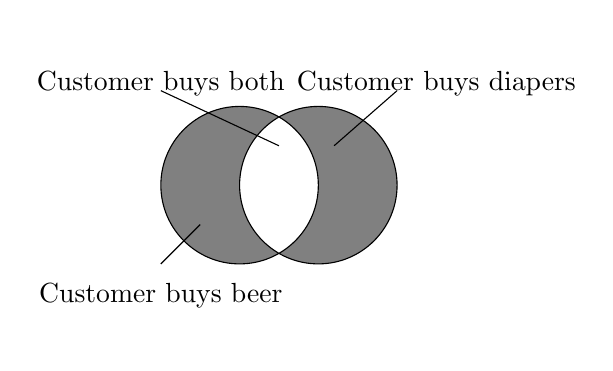
\begin{tikzpicture}[fill=gray]
				% left hand
				\scope
				\clip (-2,-2) rectangle (2,2)
				(1,0) circle (1);
				\fill (0,0) circle (1);
				\endscope
				% right hand
				\scope
				\clip (-2,-2) rectangle (2,2)
				(0,0) circle (1);
				\fill (1,0) circle (1);
				\endscope
				% outline
				\draw (0,0) circle (1) (0,1) (1,0) circle (1) (1,1);
				\node[label=below:{Customer buys beer}] at (-1,-1) {};
				\node[label=below:{Customer buys diapers}] at (2.5,1.7) {};
				\node[label=below:{Customer buys both}] at (-1,1.7) {};
				\draw (-1,-1) -- (-0.5,-0.5);
				\draw (2,1.2) -- (1.2,0.5);
				\draw (-1,1.2) -- (0.5,0.5);
			\end{tikzpicture}
		\end{column}
		\begin{column}{0.5\textwidth}
			\vspace{-1.6cm}
			\begin{itemize}
				\item \textbf{Reminder:}
				      \begin{itemize}
					      \item \textbf{Frequent Itemsets:}
					            \begin{itemize}
						            \item \textbf{1-itemsets:} \\
						                  \{Beer\}: $3$, \{Nuts\}: $3$, \{Diapers\}: $4$, \{Eggs\}: $3$
						            \item \textbf{2-itemsets:} \\
						                  \{Beer, Diapers\}: $3$
					            \end{itemize}
				      \end{itemize}
				\item \textbf{Closed Itemsets:}

				      \begin{itemize}
					      \item \textbf{1-itemsets:} \\
					            \begin{itemize}
						            \item \only<2->{\{Nuts\}: $3$, \{Diapers\}: $4$, \{Eggs\}: $3$}
					            \end{itemize}
					      \item \textbf{2-itemsets:} \\
					            \begin{itemize}
						            \item \only<3->{\{Beer, Diapers\}: $3$}
					            \end{itemize}
				      \end{itemize}
				\item \textbf{Max-Itemsets:}
				      \begin{itemize}
					      \item \textbf{1-itemsets:} \\
					            \begin{itemize}
						            \item \only<4->{\{Nuts\}: $3$, \{Eggs\}: $3$}
					            \end{itemize}
					      \item \textbf{2-itemsets:} \\
					            \begin{itemize}
						            \item \only<5->{\{Beer, Diapers\}: $3$}
					            \end{itemize}
				      \end{itemize}
			\end{itemize}
		\end{column}
	\end{columns}
\end{frame}
